% Adapted from the Overleaf AIAA Template by Yevgeniy Gorbachev, 2023-2024

\documentclass[report, wip, nodwg]{sac}
\usepackage[utf8]{inputenc}

\usepackage{siunitx, verbatim} % Text
\usepackage{graphicx, float, subcaption, longtable, tabularx} % Figures
\usepackage{multicol, multirow} % Fancier tables
\usepackage{pdflscape, pdfpages} % Page control

%%% ATTENTION EDITORS %%%%%%%%%%%%%%%%%%%%%%%%%%%%%%%
% Scroll down to the "WRITE THE REPORT" section or click on the headings in the "file outline" in the bottom-left of your screen

\newcommand\formlink[1]{\href{#1}
{http://www.soundingrocket.org/sa-cup-documents--forms.html}}

% 2024 Descriptions

\def\NomenclatureDescription
{
	Use all variables defined here. Do not define acronyms here.
}

\def\AbstractDescription
{
	At a minimum, the abstract shall identify the launch vehicles
	mission/category, identify any unique/defining characteristics, define the
	payload's mission (if applicable), and provide whatever additional
	information may be necessary to convey any other high-level project or
	program goals \& objectives.
}

\def\IntroductionDescription
{
	This section provides an overview of the academic program, stakeholders,
	team structure, and team management strategies. The introduction may repeat
	some of the content included in the abstract, because the abstract is
	intended to act as a standalone synopsis if necessary.
}

\def\SAODescription
{
    This section shall begin with a top-level overview of the integrated system,
    including a cutaway figure depicting the fully integrated launch vehicle and
    its major subsystems – configured for the mission being flown in the
    competition. This description shall be followed by the following
    subsections. Each subsection shall include detailed descriptions of each
    subsystem, and reflect the technical analyses used to support design and
    manufacturing decisions. The Project Technical Report should not just
    discuss what the team did, but the reasoning for their choices. These may
    include, but are not limited to, design goals, limitations, potential
    trade-offs, anticipated component loads along with safety factors. Technical
    drawings of these subsystems should be included in the specified appendix.
    \begin{itemize}
        \item Propulsion Subystems
        \item Aero-structures Subsystems
        \item Recovery Subsystems
        \item Payload Subsystems
    \end{itemize}
}

\def\CONOPSDescription
{
    The Project Technical Report shall contain a Mission Concept of Operations
    (CONOPS) Overview. This section shall identify the mission phases, include a
    figure, and describe the nominal operation of all subsystems during each phase
    (e.g., a description of what is supposed to be occurring in each phase, and what
    subsystem[s] are responsible for accomplishing this). Furthermore, this section
    shall define what mission events signify a phase transition has occurred (e.g.,
    "Ignition" may begin when a FIRE signal is sent to the igniter and conclude when
    the propulsion system comes up to chamber pressure. Similarly, "Liftoff" may
    begin at vehicle first motion, and conclude when the vehicle is free of the
    launch rail). Phases and phase transitions are expected to vary from system to
    system based on specific design implementations and mission goals \& objectives.
    No matter how a team defines these mission phases and phase transitions, they
    will be used to help organize failure modes identified in a Risk Assessment
    Appendix – described in Section 2.6.2.9 of this document.
}

\def\ConclusionDescription
{
    This section shall include the lessons learned during the design, manufacture,
    and testing of the project, both from a team management and technical
    development perspective. If you had failures, what did you learn from them?
    Furthermore, this section should include strategies for corporate knowledge
    transfer from senior student team members to the rising underclassmen who will
    soon take their place.
}

\def\SystemMeasuresDescription
{
The first Project Technical Report appendix shall contain System Weights,
Measures, and Performance Data. All information will be reported using Imperial
units (inches, feet, pounds, Newtons, etc.) This shall include:
\begin{enumerate}[a.]
    \item Basic rocket information, including number of stages, vehicle length,
    airframe diameter, number of fins, fin semi-span, fin tip and root chord,
    fin thickness, vehicle weight, propellant weight, empty motor case/structure
    weight, payload weight, liftoff weight, center of pressure and center of
    gravity.
    
    \item Propulsion information, including motor type, whether it is COTS or
    SRAD, COTS manufacturer and designation, motor letter classification,
    average thrust (N), total impulse (Ns) and motor burn time.
    
    \item Predicted flight data including launch rail length, liftoff
    thrust-weight ratio (X:1), rail departure velocity, minimum static margin,
    maximum acceleration (G), maximum velocity, fin flutter velocity, target,
    and predicted apogee.
    
    \item Include a flight profile graph.

    \item Recovery information, including the COTS and redundant altimeters
    used, drogue primary and backup deployment charges, drogue deployment
    altitude, drogue descent rate, main primary and backup deployment charges,
    main deployment altitude, main descent rate, shock cords and mechanical
    links.
\end{enumerate}
}

\def\TestReportsDescription
{
	The second Project Technical Report appendix shall contain applicable Test
	Reports from the minimum tests prescribed in the \formlink{IREC Design, Test,
	\& Evaluation Guide}. These reports shall appear in the following order. In the
	event any report is not applicable to the project in question, the team will
	include a page marked ``THIS PAGE INTENTIONALLY LEFT BLANK'' in its place.

	\begin{itemize}
		\item Recovery System Testing: In addition to descriptions of testing
			performed and the results thereof, teams shall include in this
			appendix a figure and supporting text describing the dual redundancy
			of recovery system electronics.
		\item SRAD Propulsion System Testing (if applicable): In addition to
			descriptions of testing performed and the results thereof, teams
			developing SRAD hybrid or liquid propulsion systems shall include in
			this appendix a fluid circuit diagram. This figure shall identify
			nominal operating pressures at various key points in the system-–
			including the fill system.
		\item SRAD Pressure Vessel Testing (if applicable).
        \item SRAD GPS Testing (if applicable)
        \item Payload Recovery System Testing (if applicable)
	\end{itemize}
}

\def\HazardAnalysisDescription
{
	This appendix shall address as applicable, hazardous material handling,
	transportation and storage procedures of propellants, and any other aspects
	of the design which pose potential hazards to operating personnel. A
	mitigation approach--by process and/or design--shall be defined for each
	hazard identified. An example of such a matrix is available on \formlink{the
	ESRA website}.
}

\def\RiskAssessmentDescription
{
	This appendix shall summarize risk and reliability concepts associated with the
	project. All identified failure modes which pose a risk to mission success
	shall be recorded in a matrix, organized according to the mission phases
	identified by the CONOPS. A mitigation approach--by process and/or
	design--shall be defined for each risk identified. An example of such a matrix
	is available on the\formlink{the ESRA website}.
}

\def\ChecklistsDescription
{
	This appendix shall include detailed checklist procedures for final
	assembly, arming, launch, and recovery operations. Furthermore, these
	checklists shall include alternate process flows for dis-arming/safeing the
	system based on identified failure modes. These off-nominal checklist
	procedures shall not conflict with the \formlink{IREC Range Standard Operating
	Procedures}. Teams developing SRAD hybrid or liquid propulsion systems shall
	also include in this appendix a description of processes and procedures used
	for cleaning all propellant tanks and other fluid circuit components.

	Competition officials will verify teams are following their checklists during
	all operations--including assembly, preflight, launch, and recovery operations.
	Therefore, teams shall maintain a complete, hardcopy set of these checklist
	procedures with their flight hardware during all range activities.Insufficient
	detail, failure to bring paper hard copies, and failure to use your team's
    detailed checklist will make your team ineligible for flight activities until
    conflicts are resolved. 
}

\def\DrawingsDescription
{
    The sixth Project Technical Report appendix shall contain detailed Engineering
    Drawings. This appendix shall include any revision controlled technical drawings
    necessary to define significant subsystems and components SRAD subsystems or
    components shall have their own respective detailed Engineering Drawings that
    are rolled up into the top level assembly. To reduce file size, please do not
    embed full CAD models – just use a picture.
}

\def\AcknowledgementsDescription
{
	An Acknowledgments section, if used, \textbf{immediately precedes} the
	References. Sponsorship information and funding data are included here. The
	preferred spelling of the word ``acknowledgment'' in American English is
	without the ``e'' after the ``g.'' Avoid expressions such as ``One of us
	(S.B.A.) would like to thank\ldots'' Instead, write ``F.~A.~Author
	thanks\ldots'' Sponsor and financial support acknowledgments are also to be
	listed in the ``acknowledgments'' section.
}


%%% TEAM LEADER: POPULATE THESE
%% Document variables %%
\sacteam{XXX}
\sacyear{YYYY}

\title{Project Technical Report Title} % Whatever you want

\author{
First A. Author\footnote{Author Title} 
and Second B. Buthor\footnote{Buthor Title}
}
\affil{Institution, Address}

%% End document variables %%

\begin{document}

\maketitle

\begin{abstract}
	\helptext{\AbstractDescription}
\end{abstract}

\section{Nomenclature}
\helptext{\NomenclatureDescription}
{
    \renewcommand\arraystretch{1.0}
	\noindent
    \begin{longtable*}{@{}p{0.3in}@{\quad=\quad}p{5.7in}@{}}
    \wiptext{ 
        \(C_\text{D}\) & Drag coefficient (EXAMPLE VARIABLE) \\	
        \(D\) & Parachute diameter (EXAMPLE VARIABLE) \\
        \(A\) & Cross-sectional area (EXAMPLE VARIABLE) \\
        \(v\) & Descent rate (EXAMPLE VARIABLE) \\ 
        \(\rho_0\) & Free-stream density at ground level (EXAMPLE VARIABLE) \\
        \(\rho\) & Free-stream density at altitude (EXAMPLE VARIABLE) \\
	}
        % ACTUAL CODE HERE
	\end{longtable*}
}

%%%% REPORT BODY
	\section{Introduction} \label{intro}
	\helptext{\IntroductionDescription}
 
	\section{System Architecture Overview} \label{sao}
	\helptext{\SAODescription}
 
	\subsection{Propulsion} \label{propulsion}

	\subsection{Aero-structures} \label{structures}

	\subsection{Recovery} \label{recovery}

	\subsection{Payload} \label{payload}
 
	\section{Mission Concept of Operations Overview} \label{conops}
 
	\helptext{\CONOPSDescription}

	\section{Conclusion and Lessons Learned}
	\helptext{\ConclusionDescription}

%%%%%%%% APPENDIX
	\appendix
    \renewcommand{\thesubsection}{\thesection.\arabic{subsection}}
    \renewcommand{\thesubsubsection}{\thesubsection.\arabic{subsubsection}}

	\wiptext{
        \section*{Formatting examples}

This section provides examples of \LaTeX{} tables, figures, equations,
lists, citations, and references to the same. This will not be compiled if
the WIP flag is not set.
\subsection*{Text}

Use \verb|\textbf{}| to \textbf{bold text}, \verb|\textit{}| to
\textit{italicize}, \verb|\verb||| for \verb|code|, or one after the other for
\textit{\textbf{both}}.
If there is no blank line or explicit newline after the previous thing, you're
in the same paragraph. Without a blank line or newline, the paragraph will be
continuous.

Blank line for a new paragraph (you know because it's automatically indented).
Two backslashes \verb|\\| \\ for a new line without a new paragraph.

Backslash open/close parentheses for inline equations \(\omega = \Omega \equiv
\sqrt{\frac{k}{m}}\). Greek letters are just their English spelling, and capital
Greek letters capitalize the first letter. Aligned non-numbered equation using
brackets:

\[f(t) = \sum_{k = 0}^{\infty} a_{n} \sin(k\omega_{0}x)\]

\subsection*{Lists}

\begin{enumerate}[(1)]
    \item \verb|\begin{enumerate}[<format>] .. \item ... \end{enumerate}| to create a list. \label{list:examples-head}

    \item This list has the format \verb|(1)|, which means it will be numbered, with parentheses surrounding the number.

    \item 
\end{enumerate}

\subsection*{Figures and tables}
Aligned numbered equation (Eq. \ref{eq:example-eq}) using \verb|begin| and \verb|end|:

\subsection*{Cross-references}

\verb|\[ ... \]| creates an aligned unlabeled equation. To make a labeled equation, create an \verb|equation| environment: 

\begin{equation} \label{eq:example-eq}
    f(t) = \sum_{k = 0}^{\infty} a_{n} \sin(k\omega_{0}x)
\end{equation}

To cite Eq. \ref{eq:example-eq}, use \verb|\ref{}|. Figures and tables each have
their own numbering, and you can refer to them with  Fig. \ref{fig:example-fig},
Table \ref{tbl:example-table}. You can also refer to list items, like item
\ref{list:examples-head}, which is the list item for creating lists.


\begin{figure}[H]
    \centering
    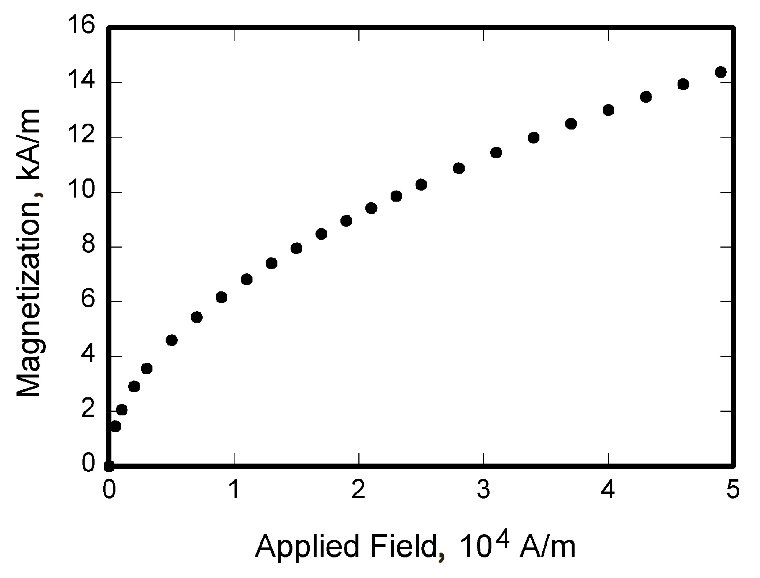
\includegraphics[width=2in]{fig/graph.jpg} % path to figure
    \caption{Magnetization as a function of applied fields} 
    \label{fig:example-fig} % how we refer to this figure's number
    % Figures must have "fig:" in the label and tables must have "tbl:" in
    % the label
\end{figure}

\begin{table}[H]
    \centering
    \caption{Informative table caption}
    % in this case, Tabular is how we express a table in LaTeX, but if we
    % had a picture of a table, we would include that using \includegraphics
    % or similar.

    % the vertical bars you put in the spec will appear - if you want two
    % columns to not be separated, omit that bar.
    \begin{tabular}{|l|cr|p{2in}|} 

        % MANDATORY: Each table row starts with "\hline" and ends with "\\"
        \hline Left column & Centered column & Right column & 2" fixed-width
        column \\
        \hline A & B & C & Lorem ipsum dolor sit amet, consectetur adipiscing elit \\
        \hline D & E & F & sed do eiusmod tempor incididunt ut labore et
        dolore magna aliqua \\
        \hline % MANDATORY: Table ends with one "\hline"
    \end{tabular}	
    \label{tbl:example-table}
\end{table}	

\paragraph{Citations} Use the \verb|cite| command to cite resources in the
\verb|.bib| file \cite{peyret2012computational, oates1997aerothermodynamics}.
	}

	\section{System Weights, Measures, and Performance Data}\label{measures}
	\helptext{\SystemMeasuresDescription}

	\pagebreak
	\section{Project Test Reports}\label{tests}
	\helptext{\TestReportsDescription}

	\subsection{Recovery System Testing}\label{test-recovery}
    \pageleftblank

	\subsection{SRAD Propulsion System Testing}\label{test-propulsion}
	\pageleftblank

	\subsection{SRAD Pressure Vessel Testing}\label{test-pressure-vessel}
	\pageleftblank

    \subsection{SRAD GPS Testing}\label{gps-test}
    \pageleftblank

	\subsection{Payload Recovery System Testing}\label{test-payload-recovery}
    \pageleftblank
    
	\begin{landscape}
		\section{Hazard Analysis}\label{hazard}
		\helptext{\HazardAnalysisDescription}

		\begingroup

\hspace{-2em}
\small
\begin{longtable}{@{}|p{1.75in}|p{2in}|p{1.75in}|p{2in}|p{0.75in}|@{}}
	\hline Hazard & Causes & Risk \& Rationale & Mitigations & Mitigated risk \\

	\hline Explosion of solid-propellant rocket motor during launch, with blast or flying debris causing injury & & & & \\

	\hline Black powder deployment charges ignite during assembly & & & & \\

	\hline Rocket deviates from nominal flight path, comes in contact with personnel at high speed & & & & \\

	\hline Recovery system fails to deploy or partially deploys, rocket or payload comes in contact with personnel & & & & \\

	\hline Recovery system deploys during assembly or prelaunch, causing injury & & & & \\

	\hline Main parachute deploys at or near apogee, rocket or payload drifts to highway(s) or restricted areas & & & & \\
 
	\hline Rocket does not ignite when command is given (“hang fire”), but does ignite when team approaches to troubleshoot & & & & \\

	\hline 

\end{longtable}
\endgroup


	\end{landscape}

    \pagebreak
    
	\begin{landscape}
		\section{Risk Assessment}\label{risk}
		\helptext{\RiskAssessmentDescription}
	\end{landscape}

	\section{Assembly, Preflight, Launch, and Recovery Checklists} \label{checklists}
	\helptext{\ChecklistsDescription}

    \pagebreak
	\section{Engineering Drawings} \label{drawings}
	\helptext{\DrawingsDescription}
    \pageleftblank

    %\putdrawings
    
	\section*{Acknowledgments}
	\helptext{\AcknowledgementsDescription}

	\bibliography{lib/bibliography}

\end{document}